% cd /storage/emulated/0/Documents/documents/latex/1920/Grade-8/3rd/inequalities-in-one-triangle/&& pdflatex hand-inequalities-in-one-triangle.tex && divide 1x2 hand-inequalities-in-one-triangle.pdf


\documentclass[handout]{beamer} 

\usepackage{pgfpages} 
\mode<handout>{%
\pgfpagesuselayout{4 on 1}[%letterpaper, 
legalpaper,% landscape, 
border shrink=1mm] 
}

\usepackage{xcolor}
\usepackage{anyfontsize}
\usepackage{enumitem}
\usepackage{multicol}
\usepackage{amsmath, makecell}
\usepackage{tabularx} 
\usepackage{gensymb}
\usepackage{wasysym} %for checked symbol 
\usepackage{multirow}
\usepackage{graphicx, tipa}
\usepackage{tikz}
\usetikzlibrary{angles,quotes}
\usepackage{pgfplots} 
\usetikzlibrary{calc}
\pgfplotsset{compat=newest}
\usetikzlibrary{arrows.meta}
\usetikzlibrary{intersections}
\usetikzlibrary{decorations.pathreplacing}
\usepackage{flafter}
%\usepackage{fourier} 
\usepackage{amsmath,amssymb,cancel,units}
\usepackage{microtype} % nicer output 
\usepackage{hfoldsty} % nicer output 
\usepackage{fixltx2e} 
\usepackage{mathptmx}
\usepackage{numprint}
\usepackage[T1]{fontenc}
\usepackage[utf8]{inputenc} 
\usepackage{stackengine} %to define \pesos 
\usepackage{lmodern} %scalable font
\usepackage{booktabs}
\usepackage{array}


\pagenumbering{gobble}
%\linespread{0.9}
\newcommand{\vspce}{\vspace{0.75ex}}

\newcommand{\hspce}{\hspace{0.5em}}

\newcommand{\blank}{\underline{\hspace{2em}}}%{\rule{1em}{0.15ex}}

\newcommand{\arc}[1]{{% 
\setbox9=\hbox{#1}% 
\ooalign{\resizebox{\wd9}{\height}{\texttoptiebar{\phantom{A}}}\cr#1}}}


\newcommand\pesos{\stackengine{-1.4ex}{P}{\stackengine{-1.25ex}{$-$}{$-$}{O}{c}{F}{F}{S}}{O}{c}{F}{T}{S}} 


\renewcommand\theadalign{bc} 

\renewcommand\theadfont{\bfseries} 

\renewcommand\theadgape{\Gape[4pt]} 

\renewcommand\cellgape{\Gape[4pt]} 

\pagenumbering{gobble}

\newcolumntype{Y}{>{\centering\arraybackslash}X} %for tabularx

\newcolumntype{R}{>{\raggedleft\arraybackslash}X} %for tabularx

\newcolumntype{Z}{>{\raggedleft\arraybackslash}X} %for tabularx

\newcolumntype{L}{>{\raggedright\arraybackslash}X} %for tabularx

\newcolumntype{A}[1]{>{\raggedright\arraybackslash}p{#1}} %for longtable LEFT

\newcolumntype{C}[1]{>{\centering\arraybackslash}p{#1}} %for longtable CENTER

\newcolumntype{B}[1]{>{\raggedleft\arraybackslash}p{#1}} %for longtable RIGHT 
 
\renewcommand{\tabularxcolumn}[1]{>{\small}m{#1}}

\newcolumntype{N}[1]{>{\raggedleft}p{#1}} %for tabular left 

\newcolumntype{M}[1]{>{\raggedright\arraybackslash}p{#1}} %for tabular right 

\newcommand{\myaxis}{xticklabels={}, 
yticklabels={}, 
ymin=-10, ymax=10,
xmin=-10, xmax=10,
axis lines = center, 
inner axis line style={Latex-Latex,very thick}, 
grid=both,
minor tick num=4, 
tick align=inside} % grid without labels, origin at the center, 10 units from origin

\newcommand{\axisfive}{xticklabels={}, 
yticklabels={}, 
ymin=-5, ymax=5,
xmin=-5, xmax=5,
axis lines = center, 
inner axis line style={Latex-Latex,very thick}, 
grid=both,
minor tick num=1, 
tick align=inside} % grid with labels, origin at the center, 5 units from origin 

\newcommand \redcheck {{\color{red}\checkmark}}



%\setbeamertemplate{itemize items}{\textbullet} 
%\useinnertheme{circles} 

%\newcommand{\vertadjust}{\vspace*{-1.5in}} % for letterpaper
%\newcommand{\vertadjustb}{\vspace*{-1.5in}} % for letterpaper
\newcommand{\vertadjust}{\vspace*{-2.5in}} % for legalpaper
\newcommand{\vertadjustb}{\vspace*{-2.5in}} % for legalpaper

\def\lenA{1.7cm}
\def\lenB{1.2cm}
\def\leninnersep{\lenA}

\begin{document} 

% frame 1
\vertadjust
\begin{frame} 
\begin{center}
\textbf{Inequalities in One Triangle 
}
\end{center}

\vspce
Unequal Sides Theorem: 
 If the lengths of the sides of a triangle are not equal, then the angles opposite these sides are also not equal and the larger angle is opposite the longer side.
 
\vspce 

Unequal Angles Theorem: If the measure of the three angles of a triangle is not equal, the sides opposite the angles are also not equal and the longer side is opposite the larger angle. 

\vspce 

Triangle Inequality Theorem: The sum of the length of the two sides of a triangle is greater than the third side.

\vspce 

The Exterior Angle Theorem 1: The measure of an exterior angle of a triangle is greater than the measure of either remote interior angle.

\vspce 

The Exterior Angle Theorem 2: The measure of the exterior angle of a triangle is equal to the sum of the measures of the two remote interior angles.  %\\
%\input{hand-inequalities-in-one-triangle-input1}
\def\figdir{/storage/emulated/0/Documents/documents/latex/1920/Grade-8/3rd/inequalities-in-one-triangle/f}

\textbf{Practice Exercises}
%\textbf{Problem Set}

\vspce

\begin{enumerate}[label = \Alph*. ]
%A
\item \hspce Arrange the angles of the triangles in increasing order. 

\begin{multicols}{2}

\begin{enumerate}[label = \arabic*. ]
%1
\item 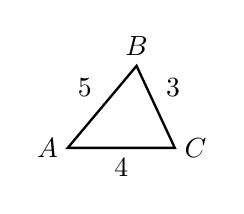
\begin{tikzpicture}

\def\len1{0.8*\lenA}

\draw[line width=0.3mm] (0,0) coordinate (a)  -- (50:\len1) coordinate (b) node[midway, anchor=south east, inner sep=0.07*\leninnersep, rotate=0] (5) {$ 5$} -- (0:\len1) coordinate (c) node[midway, anchor=south west, inner sep=0.07*\leninnersep, rotate=0] (3) {$ 3$}  -- cycle node[midway, anchor=north, inner sep=0.07*\leninnersep, rotate=0] (4) {$ 4$} ; 

\node[anchor=east, inner sep=0.07*\leninnersep, rotate=0] (a-label) at (a) {$ A$}; 

\node[anchor=south, inner sep=0.07*\leninnersep, rotate=0] (b-label) at (b) {$ B$}; 

\node[anchor=west, inner sep=0.07*\leninnersep, rotate=0] (c-label) at (c) {$ C$}; 

\end{tikzpicture} 
%2
\item 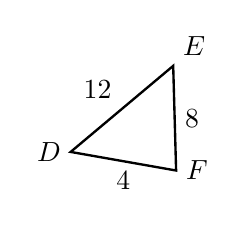
\begin{tikzpicture}

\def\len2{\lenA}

\draw[line width=0.3mm] (0,0) coordinate (d)  -- (40:\len2) coordinate (e) node[midway, anchor=south east, inner sep=0.07*\leninnersep, rotate=0] (12) {$ 12$} -- (-10:0.8*\len2) coordinate (f) node[midway, anchor=west, inner sep=0.07*\leninnersep, rotate=0] (8) {$ 8$} -- cycle node[midway, anchor=north, inner sep=0.07*\leninnersep, rotate=0] (4) {$ 4$}; 

\node[anchor=east, inner sep=0.07*\leninnersep, rotate=0] (d-label) at (d) {$ D$}; 

\node[anchor=south west, inner sep=0.07*\leninnersep, rotate=0] (e-label) at (e) {$ E$}; 

\node[anchor=west, inner sep=0.07*\leninnersep, rotate=0] (f-label) at (f) {$ F$}; 

\end{tikzpicture} 
%3
\item 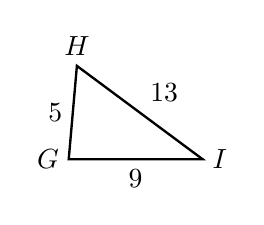
\begin{tikzpicture}

\def\len3{\lenA}

\draw[line width=0.3mm] (0,0) coordinate (g)  -- (85:0.7*\len3) coordinate (h) node[midway, anchor=east, inner sep=0.07*\leninnersep, rotate=0] (5) {$ 5$} -- (0:\len3) coordinate (i) node[midway, anchor=south west, inner sep=0.07*\leninnersep, rotate=0] (13) {$ 13$} -- cycle node[midway, anchor=north, inner sep=0.07*\leninnersep, rotate=0] (9) {$ 9$};  

\node[anchor=south, inner sep=0.07*\leninnersep, rotate=0] (h-label) at (h) {$ H$}; 

\node[anchor=east, inner sep=0.07*\leninnersep, rotate=0] (g-label) at (g) {$ G$}; 

\node[anchor=west, inner sep=0.07*\leninnersep, rotate=0] (i-label) at (i) {$ I$};

\end{tikzpicture} 
%4
\item 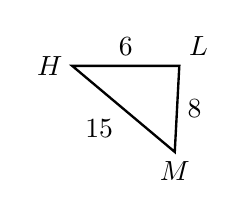
\begin{tikzpicture}

\def\len4{\lenA}

\draw[line width=0.3mm] (0,0) coordinate (h)  -- (0:0.8*\len4) coordinate (l) node[midway, anchor=south, inner sep=0.07*\leninnersep, rotate=0] (6) {$ 6$} -- (-40:\len4) coordinate (m) node[midway, anchor=west, inner sep=0.07*\leninnersep, rotate=0] (8) {$ 8$} -- cycle node[midway, anchor=north east, inner sep=0.07*\leninnersep, rotate=0] (15) {$ 15$}; 

\node[anchor=east, inner sep=0.07*\leninnersep, rotate=0] (h-label) at (h) {$ H$}; 

\node[anchor=south west, inner sep=0.07*\leninnersep, rotate=0] (l-label) at (l) {$ L$}; 

\node[anchor=north, inner sep=0.07*\leninnersep, rotate=0] (m-label) at (m) {$ M$}; 

\end{tikzpicture} 
\end{enumerate} 

\end{multicols} 
%B
\item \hspce Find the measure of the third angle of the triangle, then arrange the sides in increasing order. 

\begin{enumerate}[label = \arabic*. ]
%1
\item $m\angle{A} = 56\degree$; $ m\angle{B} = 87\degree$; $ m\angle{C} = \blank$
%2
\item $m\angle{P} = 106\degree$; $ m\angle{V} = 19\degree$; $ m\angle{C} = \blank$
%3
\item $m\angle{B} = 29\degree$; $ m\angle{P} = 72\degree$; $ m\angle{F} = \blank$
%4
\item $m\angle{G} = 97\degree$; $ m\angle{E} = 64\degree$; $ m\angle{O} = \blank$
%5
\item $m\angle{M} = 68\degree$; $ m\angle{A} = 22\degree$; $ m\angle{T} = \blank $
\end{enumerate} 
%C
\item \hspce Write \emph{Yes} if the given measure can form a triangle or \emph{No} if not. 

\vspace*{-0.75ex}

\begin{multicols}{2}

\begin{enumerate}[label = \arabic*. ]
%1
\item \hspce $8, 14, 9$
%2
\item \hspce $13, 25, 12$
%3
\item \hspce $3.6, 4.8, 9.0$
%4
\item \hspce $15, 20, 36$
%5
\item \hspce $6.5, 9.6, 2.9$ 

\end{enumerate}  

\end{multicols}



\end{enumerate} 


%\def\figdir{/storage/emulated/0/Documents/documents/latex/1920/Grade-8/3rd/inequalities-in-one-triangle/f}


\begin{enumerate}[label = \arabic*. ]
%D
\item[D. ] \hspce Give the range of the possible length of the third side of $\triangle ABC$. 

\vspace*{5ex}\hspace*{17em}\begin{tikzpicture}[remember picture, overlay] 

\def\len1{\lenA}

\draw[line width=0.3mm] (0,0) coordinate (b)  -- (50:0.6*\len1) coordinate (a) node[midway, anchor=south east, inner sep=0.07*\leninnersep, rotate=0] (c-mid) {$ c$} -- (0:\len1) coordinate (c) node[midway, anchor=south west, inner sep=0.07*\leninnersep, rotate=0] (b-mid) {$ b$} -- cycle node[midway, anchor=north, inner sep=0.07*\leninnersep, rotate=0] (a-mid) {$ a$}; 

\node[anchor=south, inner sep=0.07*\leninnersep, rotate=0] (a-label) at (a) {$ A$};

\node[anchor=east, inner sep=0.07*\leninnersep, rotate=0] (b-label) at (b) {$ B$};

\node[anchor=west, inner sep=0.07*\leninnersep, rotate=0] (c-label) at (c) {$ C$}; 

\end{tikzpicture} 
\vspace*{-7ex}

$
\begin{array}{llll}
1. \phantom{i} & a=9 & \phantom{mn} & b=7 \\
2. &	b=12 &	& c=29\\
3. &	a=15.2 &	& b=19.8 \\
4. & a=128.25 & & c=74.5 \\
5. &	a=3 \displaystyle \frac{2}{5} &	& c=2 \displaystyle \frac{1}{2}\\
\end{array}
$

%E
\item[E. ] \hspce Find the measure of the indicated angle. 
\begin{enumerate}[label = \arabic*. ]
%1
\item $m\angle{1} = 48\degree$; $m\angle{2} = 46\degree$; $ m\angle{4} = \blank$
%2
\item $m\angle{1} = 29\degree$; $ m\angle{2} = 52\degree$; $ m\angle{4} = \blank$
%3
\item $m\angle{2} = 18\degree$; $ m\angle{4} = 127\degree$; $ m\angle{1} = \blank$
%4
\item $m\angle{4} = 109\degree$; $ m\angle{1} = 86\degree$; $ m\angle{2} = \blank$
%5 
\item $m\angle{1} = (x+5)\degree$; $ m\angle{2} = (2x+51)\degree$; $ m\angle{4} = (5x-10)\degree$; $ x = \blank$
\end{enumerate}  
\end{enumerate}   

%\begin{center}

\vspace*{-19ex}\hspace*{22em}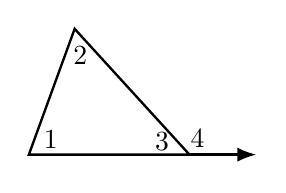
\begin{tikzpicture}

\def\len2{\lenA}

\draw[line width=0.3mm] (0,0) coordinate (1) node[yshift=-0.07*\leninnersep, inner sep=5pt, rotate=0, anchor=south west] (1-label) {$ 1$} -- (70:\len2) coordinate (2) node[xshift=2pt, inner sep=6pt, rotate=0, anchor=north] (2-label) {$ 2$} -- (0:1.2*\len2) coordinate (3) edge[-Latex] (0:1.7*\len2) node[yshift=-4pt, xshift=-2pt, inner sep=5pt, rotate=0, anchor=south east] (3-label) {$ 3$} node[yshift=0pt, xshift=-2pt, inner sep=2pt, rotate=0, anchor=south west] (4-label) {$ 4$}  -- cycle;  

\end{tikzpicture} 
\vspace*{4ex}

%\end{center} 
%\vspace*{1ex}
%\def\figdir{/storage/emulated/0/Documents/documents/latex/1920/Grade-8/3rd/inequalities-in-one-triangle/f}


%\textbf{Practice Exercises}
\textbf{Problem Set}

\vspce

\begin{enumerate}[label = \Alph*. ]
%A
\item \hspce Arrange the angles of the triangles in increasing order. 

\begin{multicols}{2}

\begin{enumerate}[label = \arabic*. ]
%1
\item 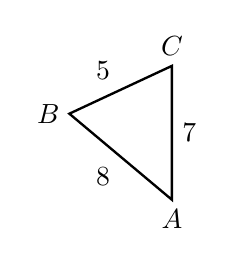
\begin{tikzpicture}

\def\len1{\lenA}

\draw[line width=0.3mm, rotate=90] (0,0) coordinate (a)  -- (50:\len1) coordinate (b) node[midway, anchor=north east, inner sep=0.07*\leninnersep, rotate=0] (8) {$ 8$} -- (0:\len1) coordinate (c) node[midway, anchor=south east, inner sep=0.07*\leninnersep, rotate=0] (5) {$ 5$}  -- cycle node[midway, anchor=west, inner sep=0.07*\leninnersep, rotate=0] (7) {$ 7$} ; 

\node[anchor=north, inner sep=0.07*\leninnersep, rotate=0] (a-label) at (a) {$ A$}; 

\node[anchor=east, inner sep=0.07*\leninnersep, rotate=0] (b-label) at (b) {$ B$}; 

\node[anchor=south, inner sep=0.07*\leninnersep, rotate=0] (c-label) at (c) {$ C$}; 

\end{tikzpicture} 
%2
\item 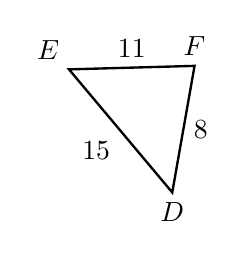
\begin{tikzpicture}

\def\len2{1.2*\lenA}

\draw[line width=0.3mm, rotate=90] (0,0) coordinate (d)  -- (40:\len2) coordinate (e) node[midway, anchor=north east, inner sep=0.07*\leninnersep, rotate=0] (15) {$ 15$} -- (-10:0.8*\len2) coordinate (f) node[midway, anchor=south, inner sep=0.07*\leninnersep, rotate=0] (11) {$ 11$} -- cycle node[midway, anchor=west, inner sep=0.07*\leninnersep, rotate=0] (4) {$ 8$}; 

\node[anchor=north, inner sep=0.07*\leninnersep, rotate=0] (d-label) at (d) {$ D$}; 

\node[anchor=south east, inner sep=0.07*\leninnersep, rotate=0] (e-label) at (e) {$ E$}; 

\node[anchor=south, inner sep=0.07*\leninnersep, rotate=0] (f-label) at (f) {$ F$}; 

\end{tikzpicture} 
%3
%\item 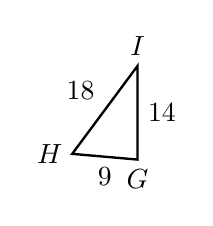
\begin{tikzpicture}

\def\len3{0.7*\lenA}

\draw[line width=0.3mm, rotate=90] (0,0) coordinate (g)  -- (85:0.7*\len3) coordinate (h) node[midway, anchor=north, inner sep=0.07*\leninnersep, rotate=0] (9) {$ 9$} -- (0:\len3) coordinate (i) node[midway, anchor=south east, inner sep=0.07*\leninnersep, rotate=0] (18) {$ 18$} -- cycle node[midway, anchor=west, inner sep=0.07*\leninnersep, rotate=0] (14) {$ 14$};  

\node[anchor=east, inner sep=0.07*\leninnersep, rotate=0] (h-label) at (h) {$ H$}; 

\node[anchor=north, inner sep=0.07*\leninnersep, rotate=0] (g-label) at (g) {$ G$}; 

\node[anchor=south, inner sep=0.07*\leninnersep, rotate=0] (i-label) at (i) {$ I$};

\end{tikzpicture} 
%4
%\item 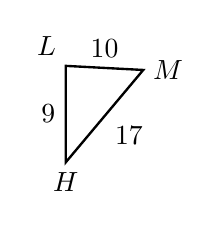
\begin{tikzpicture}

\def\len4{0.9*\lenA}

\draw[line width=0.3mm, rotate=90] (0,0) coordinate (h)  -- (0:0.8*\len4) coordinate (l) node[midway, anchor=east, inner sep=0.07*\leninnersep, rotate=0] (9) {$ 9$} -- (-40:\len4) coordinate (m) node[midway, anchor=south, inner sep=0.07*\leninnersep, rotate=0] (10) {$ 10$} -- cycle node[midway, anchor=north west, inner sep=0.07*\leninnersep, rotate=0] (17) {$ 17$}; 

\node[anchor=north, inner sep=0.07*\leninnersep, rotate=0] (h-label) at (h) {$ H$}; 

\node[anchor=south east, inner sep=0.07*\leninnersep, rotate=0] (l-label) at (l) {$ L$}; 

\node[anchor=west, inner sep=0.07*\leninnersep, rotate=0] (m-label) at (m) {$ M$}; 

\end{tikzpicture} 
\end{enumerate} 

\end{multicols} 
%B
\item \hspce Find the measure of the third angle of the triangle, then arrange the sides in increasing order. 

\begin{enumerate}[label = \arabic*. ]
%1
\item $m\angle{A} = 40\degree$; $ m\angle{B} = 89\degree$; $ m\angle{C} = \blank$
%2
\item $m\angle{P} = 117\degree$; $ m\angle{V} = 27\degree$; $ m\angle{C} = \blank$
%3
\item $m\angle{B} = 38\degree$; $ m\angle{P} = 92\degree$; $ m\angle{F} = \blank$
%4
%\item $m\angle{G} = 88\degree$; $ m\angle{E} = 71\degree$; $ m\angle{O} = \blank$
%5
%\item $m\angle{M} = 79\degree$; $ m\angle{A} = 35\degree$; $ m\angle{T} = \blank $
\end{enumerate} 
%C
\item \hspce Write \emph{Yes} if the given measure can form a triangle or \emph{No} if not. 

\vspace*{-0.75ex}

\begin{multicols}{3}

\begin{enumerate}[label = \arabic*. ]
%1
\item \hspce $6, 17, 12$
%2
\item \hspce $14, 33, 19$
%3
\item \hspce $3.7, 5.2, 8.5$
%4
%\item \hspce $27, 34, 49$
%5
%\item \hspce $6.5, 10.1, 3.6$ 

\end{enumerate}  

\end{multicols}

%D
\item \hspce Give the range of the possible length of the third side of $\triangle ABC$. 

\vspace*{4ex}\hspace*{15em}\begin{tikzpicture}[remember picture, overlay] 

\def\len1{\lenA}

\draw[line width=0.3mm] (0,0) coordinate (b)  -- (50:0.6*\len1) coordinate (a) node[midway, anchor=south east, inner sep=0.07*\leninnersep, rotate=0] (c-mid) {$ c$} -- (0:\len1) coordinate (c) node[midway, anchor=south west, inner sep=0.07*\leninnersep, rotate=0] (b-mid) {$ b$} -- cycle node[midway, anchor=north, inner sep=0.07*\leninnersep, rotate=0] (a-mid) {$ a$}; 

\node[anchor=south, inner sep=0.07*\leninnersep, rotate=0] (a-label) at (a) {$ A$};

\node[anchor=east, inner sep=0.07*\leninnersep, rotate=0] (b-label) at (b) {$ B$};

\node[anchor=west, inner sep=0.07*\leninnersep, rotate=0] (c-label) at (c) {$ C$}; 

\end{tikzpicture} 
\vspace*{-6ex}


$
\begin{array}{llll}
1. \phantom{i} & a=5 & \phantom{mn} & b=12 \\
%2. &	b=18 &	& c=23\\
2. &	a=17.4 &	& b=28.1 \\
%4. & a=107.4 & & c=74.35 \\
3. &	a=7 \displaystyle \frac{1}{4} &	& c=3 \displaystyle \frac{1}{2}\\
\end{array}
$

%E
\item \hspce Find the measure of the indicated angle. 
\begin{enumerate}[label = \arabic*. ]
%1
\item $m\angle{1} = 57\degree$; $m\angle{2} = 54\degree$; $ m\angle{4} = \blank$
%2
%\item $m\angle{1} = 43\degree$; $ m\angle{2} = 65\degree$; $ m\angle{4} = \blank$
%3
\item $m\angle{2} = 37\degree$; $ m\angle{4} = 150\degree$; $ m\angle{1} = \blank$
%4
%\item $m\angle{4} = 132\degree$; $ m\angle{1} = 76\degree$; $ m\angle{2} = \blank$
%5 
\item $m\angle{1} = (2x+7)\degree$; $ m\angle{2} = (x+31)\degree$; $ m\angle{4} = (6x-4)\degree$; $ x = \blank$
\end{enumerate}  

\end{enumerate} 

\vspace*{-16ex}\hspace*{22em}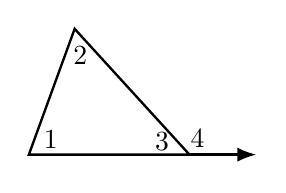
\begin{tikzpicture}

\def\len2{\lenA}

\draw[line width=0.3mm] (0,0) coordinate (1) node[yshift=-0.07*\leninnersep, inner sep=5pt, rotate=0, anchor=south west] (1-label) {$ 1$} -- (70:\len2) coordinate (2) node[xshift=2pt, inner sep=6pt, rotate=0, anchor=north] (2-label) {$ 2$} -- (0:1.2*\len2) coordinate (3) edge[-Latex] (0:1.7*\len2) node[yshift=-4pt, xshift=-2pt, inner sep=5pt, rotate=0, anchor=south east] (3-label) {$ 3$} node[yshift=0pt, xshift=-2pt, inner sep=2pt, rotate=0, anchor=south west] (4-label) {$ 4$}  -- cycle;  

\end{tikzpicture} 
\vspace*{4ex}

\end{frame}

% frame 2
\vertadjust
\begin{frame} 
%\begin{center}
\textbf{Inequalities in One Triangle 
}
\end{center}

\vspce
Unequal Sides Theorem: 
 If the lengths of the sides of a triangle are not equal, then the angles opposite these sides are also not equal and the larger angle is opposite the longer side.
 
\vspce 

Unequal Angles Theorem: If the measure of the three angles of a triangle is not equal, the sides opposite the angles are also not equal and the longer side is opposite the larger angle. 

\vspce 

Triangle Inequality Theorem: The sum of the length of the two sides of a triangle is greater than the third side.

\vspce 

The Exterior Angle Theorem 1: The measure of an exterior angle of a triangle is greater than the measure of either remote interior angle.

\vspce 

The Exterior Angle Theorem 2: The measure of the exterior angle of a triangle is equal to the sum of the measures of the two remote interior angles. % \\
%\def\figdir{/storage/emulated/0/Documents/documents/latex/1920/Grade-8/3rd/inequalities-in-one-triangle/f}

\textbf{Practice Exercises}
%\textbf{Problem Set}

\vspce

\begin{enumerate}[label = \Alph*. ]
%A
\item \hspce Arrange the angles of the triangles in increasing order. 

\begin{multicols}{2}

\begin{enumerate}[label = \arabic*. ]
%1
\item 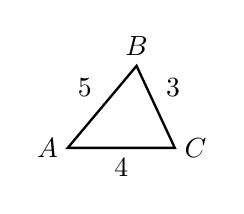
\begin{tikzpicture}

\def\len1{0.8*\lenA}

\draw[line width=0.3mm] (0,0) coordinate (a)  -- (50:\len1) coordinate (b) node[midway, anchor=south east, inner sep=0.07*\leninnersep, rotate=0] (5) {$ 5$} -- (0:\len1) coordinate (c) node[midway, anchor=south west, inner sep=0.07*\leninnersep, rotate=0] (3) {$ 3$}  -- cycle node[midway, anchor=north, inner sep=0.07*\leninnersep, rotate=0] (4) {$ 4$} ; 

\node[anchor=east, inner sep=0.07*\leninnersep, rotate=0] (a-label) at (a) {$ A$}; 

\node[anchor=south, inner sep=0.07*\leninnersep, rotate=0] (b-label) at (b) {$ B$}; 

\node[anchor=west, inner sep=0.07*\leninnersep, rotate=0] (c-label) at (c) {$ C$}; 

\end{tikzpicture} 
%2
\item 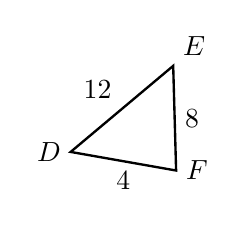
\begin{tikzpicture}

\def\len2{\lenA}

\draw[line width=0.3mm] (0,0) coordinate (d)  -- (40:\len2) coordinate (e) node[midway, anchor=south east, inner sep=0.07*\leninnersep, rotate=0] (12) {$ 12$} -- (-10:0.8*\len2) coordinate (f) node[midway, anchor=west, inner sep=0.07*\leninnersep, rotate=0] (8) {$ 8$} -- cycle node[midway, anchor=north, inner sep=0.07*\leninnersep, rotate=0] (4) {$ 4$}; 

\node[anchor=east, inner sep=0.07*\leninnersep, rotate=0] (d-label) at (d) {$ D$}; 

\node[anchor=south west, inner sep=0.07*\leninnersep, rotate=0] (e-label) at (e) {$ E$}; 

\node[anchor=west, inner sep=0.07*\leninnersep, rotate=0] (f-label) at (f) {$ F$}; 

\end{tikzpicture} 
%3
\item 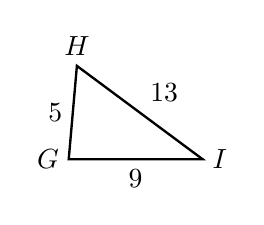
\begin{tikzpicture}

\def\len3{\lenA}

\draw[line width=0.3mm] (0,0) coordinate (g)  -- (85:0.7*\len3) coordinate (h) node[midway, anchor=east, inner sep=0.07*\leninnersep, rotate=0] (5) {$ 5$} -- (0:\len3) coordinate (i) node[midway, anchor=south west, inner sep=0.07*\leninnersep, rotate=0] (13) {$ 13$} -- cycle node[midway, anchor=north, inner sep=0.07*\leninnersep, rotate=0] (9) {$ 9$};  

\node[anchor=south, inner sep=0.07*\leninnersep, rotate=0] (h-label) at (h) {$ H$}; 

\node[anchor=east, inner sep=0.07*\leninnersep, rotate=0] (g-label) at (g) {$ G$}; 

\node[anchor=west, inner sep=0.07*\leninnersep, rotate=0] (i-label) at (i) {$ I$};

\end{tikzpicture} 
%4
\item 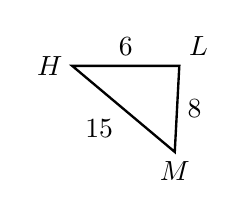
\begin{tikzpicture}

\def\len4{\lenA}

\draw[line width=0.3mm] (0,0) coordinate (h)  -- (0:0.8*\len4) coordinate (l) node[midway, anchor=south, inner sep=0.07*\leninnersep, rotate=0] (6) {$ 6$} -- (-40:\len4) coordinate (m) node[midway, anchor=west, inner sep=0.07*\leninnersep, rotate=0] (8) {$ 8$} -- cycle node[midway, anchor=north east, inner sep=0.07*\leninnersep, rotate=0] (15) {$ 15$}; 

\node[anchor=east, inner sep=0.07*\leninnersep, rotate=0] (h-label) at (h) {$ H$}; 

\node[anchor=south west, inner sep=0.07*\leninnersep, rotate=0] (l-label) at (l) {$ L$}; 

\node[anchor=north, inner sep=0.07*\leninnersep, rotate=0] (m-label) at (m) {$ M$}; 

\end{tikzpicture} 
\end{enumerate} 

\end{multicols} 
%B
\item \hspce Find the measure of the third angle of the triangle, then arrange the sides in increasing order. 

\begin{enumerate}[label = \arabic*. ]
%1
\item $m\angle{A} = 56\degree$; $ m\angle{B} = 87\degree$; $ m\angle{C} = \blank$
%2
\item $m\angle{P} = 106\degree$; $ m\angle{V} = 19\degree$; $ m\angle{C} = \blank$
%3
\item $m\angle{B} = 29\degree$; $ m\angle{P} = 72\degree$; $ m\angle{F} = \blank$
%4
\item $m\angle{G} = 97\degree$; $ m\angle{E} = 64\degree$; $ m\angle{O} = \blank$
%5
\item $m\angle{M} = 68\degree$; $ m\angle{A} = 22\degree$; $ m\angle{T} = \blank $
\end{enumerate} 
%C
\item \hspce Write \emph{Yes} if the given measure can form a triangle or \emph{No} if not. 

\vspace*{-0.75ex}

\begin{multicols}{2}

\begin{enumerate}[label = \arabic*. ]
%1
\item \hspce $8, 14, 9$
%2
\item \hspce $13, 25, 12$
%3
\item \hspce $3.6, 4.8, 9.0$
%4
\item \hspce $15, 20, 36$
%5
\item \hspce $6.5, 9.6, 2.9$ 

\end{enumerate}  

\end{multicols}



\end{enumerate} 


\def\figdir{/storage/emulated/0/Documents/documents/latex/1920/Grade-8/3rd/inequalities-in-one-triangle/f}


\begin{enumerate}[label = \arabic*. ]
%D
\item[D. ] \hspce Give the range of the possible length of the third side of $\triangle ABC$. 

\vspace*{5ex}\hspace*{17em}\begin{tikzpicture}[remember picture, overlay] 

\def\len1{\lenA}

\draw[line width=0.3mm] (0,0) coordinate (b)  -- (50:0.6*\len1) coordinate (a) node[midway, anchor=south east, inner sep=0.07*\leninnersep, rotate=0] (c-mid) {$ c$} -- (0:\len1) coordinate (c) node[midway, anchor=south west, inner sep=0.07*\leninnersep, rotate=0] (b-mid) {$ b$} -- cycle node[midway, anchor=north, inner sep=0.07*\leninnersep, rotate=0] (a-mid) {$ a$}; 

\node[anchor=south, inner sep=0.07*\leninnersep, rotate=0] (a-label) at (a) {$ A$};

\node[anchor=east, inner sep=0.07*\leninnersep, rotate=0] (b-label) at (b) {$ B$};

\node[anchor=west, inner sep=0.07*\leninnersep, rotate=0] (c-label) at (c) {$ C$}; 

\end{tikzpicture} 
\vspace*{-7ex}

$
\begin{array}{llll}
1. \phantom{i} & a=9 & \phantom{mn} & b=7 \\
2. &	b=12 &	& c=29\\
3. &	a=15.2 &	& b=19.8 \\
4. & a=128.25 & & c=74.5 \\
5. &	a=3 \displaystyle \frac{2}{5} &	& c=2 \displaystyle \frac{1}{2}\\
\end{array}
$

%E
\item[E. ] \hspce Find the measure of the indicated angle. 
\begin{enumerate}[label = \arabic*. ]
%1
\item $m\angle{1} = 48\degree$; $m\angle{2} = 46\degree$; $ m\angle{4} = \blank$
%2
\item $m\angle{1} = 29\degree$; $ m\angle{2} = 52\degree$; $ m\angle{4} = \blank$
%3
\item $m\angle{2} = 18\degree$; $ m\angle{4} = 127\degree$; $ m\angle{1} = \blank$
%4
\item $m\angle{4} = 109\degree$; $ m\angle{1} = 86\degree$; $ m\angle{2} = \blank$
%5 
\item $m\angle{1} = (x+5)\degree$; $ m\angle{2} = (2x+51)\degree$; $ m\angle{4} = (5x-10)\degree$; $ x = \blank$
\end{enumerate}  
\end{enumerate}   

%\begin{center}

\vspace*{-19ex}\hspace*{22em}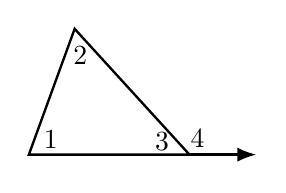
\begin{tikzpicture}

\def\len2{\lenA}

\draw[line width=0.3mm] (0,0) coordinate (1) node[yshift=-0.07*\leninnersep, inner sep=5pt, rotate=0, anchor=south west] (1-label) {$ 1$} -- (70:\len2) coordinate (2) node[xshift=2pt, inner sep=6pt, rotate=0, anchor=north] (2-label) {$ 2$} -- (0:1.2*\len2) coordinate (3) edge[-Latex] (0:1.7*\len2) node[yshift=-4pt, xshift=-2pt, inner sep=5pt, rotate=0, anchor=south east] (3-label) {$ 3$} node[yshift=0pt, xshift=-2pt, inner sep=2pt, rotate=0, anchor=south west] (4-label) {$ 4$}  -- cycle;  

\end{tikzpicture} 
\vspace*{4ex}

%\end{center} 
%\input{hand-inequalities-in-one-triangle-input2}
\vspace*{1ex}
\def\figdir{/storage/emulated/0/Documents/documents/latex/1920/Grade-8/3rd/inequalities-in-one-triangle/f}


%\textbf{Practice Exercises}
\textbf{Problem Set}

\vspce

\begin{enumerate}[label = \Alph*. ]
%A
\item \hspce Arrange the angles of the triangles in increasing order. 

\begin{multicols}{2}

\begin{enumerate}[label = \arabic*. ]
%1
\item 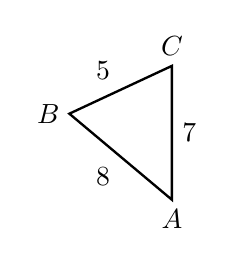
\begin{tikzpicture}

\def\len1{\lenA}

\draw[line width=0.3mm, rotate=90] (0,0) coordinate (a)  -- (50:\len1) coordinate (b) node[midway, anchor=north east, inner sep=0.07*\leninnersep, rotate=0] (8) {$ 8$} -- (0:\len1) coordinate (c) node[midway, anchor=south east, inner sep=0.07*\leninnersep, rotate=0] (5) {$ 5$}  -- cycle node[midway, anchor=west, inner sep=0.07*\leninnersep, rotate=0] (7) {$ 7$} ; 

\node[anchor=north, inner sep=0.07*\leninnersep, rotate=0] (a-label) at (a) {$ A$}; 

\node[anchor=east, inner sep=0.07*\leninnersep, rotate=0] (b-label) at (b) {$ B$}; 

\node[anchor=south, inner sep=0.07*\leninnersep, rotate=0] (c-label) at (c) {$ C$}; 

\end{tikzpicture} 
%2
\item 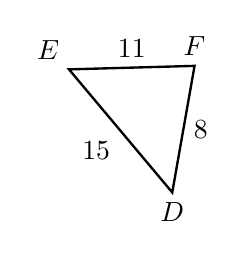
\begin{tikzpicture}

\def\len2{1.2*\lenA}

\draw[line width=0.3mm, rotate=90] (0,0) coordinate (d)  -- (40:\len2) coordinate (e) node[midway, anchor=north east, inner sep=0.07*\leninnersep, rotate=0] (15) {$ 15$} -- (-10:0.8*\len2) coordinate (f) node[midway, anchor=south, inner sep=0.07*\leninnersep, rotate=0] (11) {$ 11$} -- cycle node[midway, anchor=west, inner sep=0.07*\leninnersep, rotate=0] (4) {$ 8$}; 

\node[anchor=north, inner sep=0.07*\leninnersep, rotate=0] (d-label) at (d) {$ D$}; 

\node[anchor=south east, inner sep=0.07*\leninnersep, rotate=0] (e-label) at (e) {$ E$}; 

\node[anchor=south, inner sep=0.07*\leninnersep, rotate=0] (f-label) at (f) {$ F$}; 

\end{tikzpicture} 
%3
%\item 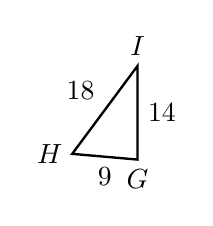
\begin{tikzpicture}

\def\len3{0.7*\lenA}

\draw[line width=0.3mm, rotate=90] (0,0) coordinate (g)  -- (85:0.7*\len3) coordinate (h) node[midway, anchor=north, inner sep=0.07*\leninnersep, rotate=0] (9) {$ 9$} -- (0:\len3) coordinate (i) node[midway, anchor=south east, inner sep=0.07*\leninnersep, rotate=0] (18) {$ 18$} -- cycle node[midway, anchor=west, inner sep=0.07*\leninnersep, rotate=0] (14) {$ 14$};  

\node[anchor=east, inner sep=0.07*\leninnersep, rotate=0] (h-label) at (h) {$ H$}; 

\node[anchor=north, inner sep=0.07*\leninnersep, rotate=0] (g-label) at (g) {$ G$}; 

\node[anchor=south, inner sep=0.07*\leninnersep, rotate=0] (i-label) at (i) {$ I$};

\end{tikzpicture} 
%4
%\item 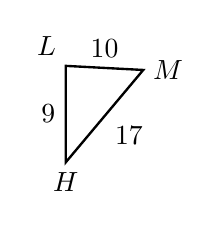
\begin{tikzpicture}

\def\len4{0.9*\lenA}

\draw[line width=0.3mm, rotate=90] (0,0) coordinate (h)  -- (0:0.8*\len4) coordinate (l) node[midway, anchor=east, inner sep=0.07*\leninnersep, rotate=0] (9) {$ 9$} -- (-40:\len4) coordinate (m) node[midway, anchor=south, inner sep=0.07*\leninnersep, rotate=0] (10) {$ 10$} -- cycle node[midway, anchor=north west, inner sep=0.07*\leninnersep, rotate=0] (17) {$ 17$}; 

\node[anchor=north, inner sep=0.07*\leninnersep, rotate=0] (h-label) at (h) {$ H$}; 

\node[anchor=south east, inner sep=0.07*\leninnersep, rotate=0] (l-label) at (l) {$ L$}; 

\node[anchor=west, inner sep=0.07*\leninnersep, rotate=0] (m-label) at (m) {$ M$}; 

\end{tikzpicture} 
\end{enumerate} 

\end{multicols} 
%B
\item \hspce Find the measure of the third angle of the triangle, then arrange the sides in increasing order. 

\begin{enumerate}[label = \arabic*. ]
%1
\item $m\angle{A} = 40\degree$; $ m\angle{B} = 89\degree$; $ m\angle{C} = \blank$
%2
\item $m\angle{P} = 117\degree$; $ m\angle{V} = 27\degree$; $ m\angle{C} = \blank$
%3
\item $m\angle{B} = 38\degree$; $ m\angle{P} = 92\degree$; $ m\angle{F} = \blank$
%4
%\item $m\angle{G} = 88\degree$; $ m\angle{E} = 71\degree$; $ m\angle{O} = \blank$
%5
%\item $m\angle{M} = 79\degree$; $ m\angle{A} = 35\degree$; $ m\angle{T} = \blank $
\end{enumerate} 
%C
\item \hspce Write \emph{Yes} if the given measure can form a triangle or \emph{No} if not. 

\vspace*{-0.75ex}

\begin{multicols}{3}

\begin{enumerate}[label = \arabic*. ]
%1
\item \hspce $6, 17, 12$
%2
\item \hspce $14, 33, 19$
%3
\item \hspce $3.7, 5.2, 8.5$
%4
%\item \hspce $27, 34, 49$
%5
%\item \hspce $6.5, 10.1, 3.6$ 

\end{enumerate}  

\end{multicols}

%D
\item \hspce Give the range of the possible length of the third side of $\triangle ABC$. 

\vspace*{4ex}\hspace*{15em}\begin{tikzpicture}[remember picture, overlay] 

\def\len1{\lenA}

\draw[line width=0.3mm] (0,0) coordinate (b)  -- (50:0.6*\len1) coordinate (a) node[midway, anchor=south east, inner sep=0.07*\leninnersep, rotate=0] (c-mid) {$ c$} -- (0:\len1) coordinate (c) node[midway, anchor=south west, inner sep=0.07*\leninnersep, rotate=0] (b-mid) {$ b$} -- cycle node[midway, anchor=north, inner sep=0.07*\leninnersep, rotate=0] (a-mid) {$ a$}; 

\node[anchor=south, inner sep=0.07*\leninnersep, rotate=0] (a-label) at (a) {$ A$};

\node[anchor=east, inner sep=0.07*\leninnersep, rotate=0] (b-label) at (b) {$ B$};

\node[anchor=west, inner sep=0.07*\leninnersep, rotate=0] (c-label) at (c) {$ C$}; 

\end{tikzpicture} 
\vspace*{-6ex}


$
\begin{array}{llll}
1. \phantom{i} & a=5 & \phantom{mn} & b=12 \\
%2. &	b=18 &	& c=23\\
2. &	a=17.4 &	& b=28.1 \\
%4. & a=107.4 & & c=74.35 \\
3. &	a=7 \displaystyle \frac{1}{4} &	& c=3 \displaystyle \frac{1}{2}\\
\end{array}
$

%E
\item \hspce Find the measure of the indicated angle. 
\begin{enumerate}[label = \arabic*. ]
%1
\item $m\angle{1} = 57\degree$; $m\angle{2} = 54\degree$; $ m\angle{4} = \blank$
%2
%\item $m\angle{1} = 43\degree$; $ m\angle{2} = 65\degree$; $ m\angle{4} = \blank$
%3
\item $m\angle{2} = 37\degree$; $ m\angle{4} = 150\degree$; $ m\angle{1} = \blank$
%4
%\item $m\angle{4} = 132\degree$; $ m\angle{1} = 76\degree$; $ m\angle{2} = \blank$
%5 
\item $m\angle{1} = (2x+7)\degree$; $ m\angle{2} = (x+31)\degree$; $ m\angle{4} = (6x-4)\degree$; $ x = \blank$
\end{enumerate}  

\end{enumerate} 

\vspace*{-16ex}\hspace*{22em}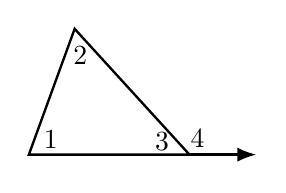
\begin{tikzpicture}

\def\len2{\lenA}

\draw[line width=0.3mm] (0,0) coordinate (1) node[yshift=-0.07*\leninnersep, inner sep=5pt, rotate=0, anchor=south west] (1-label) {$ 1$} -- (70:\len2) coordinate (2) node[xshift=2pt, inner sep=6pt, rotate=0, anchor=north] (2-label) {$ 2$} -- (0:1.2*\len2) coordinate (3) edge[-Latex] (0:1.7*\len2) node[yshift=-4pt, xshift=-2pt, inner sep=5pt, rotate=0, anchor=south east] (3-label) {$ 3$} node[yshift=0pt, xshift=-2pt, inner sep=2pt, rotate=0, anchor=south west] (4-label) {$ 4$}  -- cycle;  

\end{tikzpicture} 
\vspace*{4ex}

\end{frame}

% frame 3
\vertadjustb
\begin{frame} 
\begin{center}
\textbf{Inequalities in One Triangle 
}
\end{center}

\vspce
Unequal Sides Theorem: 
 If the lengths of the sides of a triangle are not equal, then the angles opposite these sides are also not equal and the larger angle is opposite the longer side.
 
\vspce 

Unequal Angles Theorem: If the measure of the three angles of a triangle is not equal, the sides opposite the angles are also not equal and the longer side is opposite the larger angle. 

\vspce 

Triangle Inequality Theorem: The sum of the length of the two sides of a triangle is greater than the third side.

\vspce 

The Exterior Angle Theorem 1: The measure of an exterior angle of a triangle is greater than the measure of either remote interior angle.

\vspce 

The Exterior Angle Theorem 2: The measure of the exterior angle of a triangle is equal to the sum of the measures of the two remote interior angles.  
\def\figdir{/storage/emulated/0/Documents/documents/latex/1920/Grade-8/3rd/inequalities-in-one-triangle/f}

\textbf{Practice Exercises}
%\textbf{Problem Set}

\vspce

\begin{enumerate}[label = \Alph*. ]
%A
\item \hspce Arrange the angles of the triangles in increasing order. 

\begin{multicols}{2}

\begin{enumerate}[label = \arabic*. ]
%1
\item 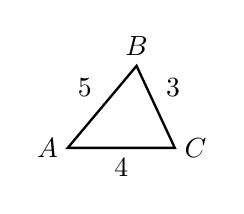
\begin{tikzpicture}

\def\len1{0.8*\lenA}

\draw[line width=0.3mm] (0,0) coordinate (a)  -- (50:\len1) coordinate (b) node[midway, anchor=south east, inner sep=0.07*\leninnersep, rotate=0] (5) {$ 5$} -- (0:\len1) coordinate (c) node[midway, anchor=south west, inner sep=0.07*\leninnersep, rotate=0] (3) {$ 3$}  -- cycle node[midway, anchor=north, inner sep=0.07*\leninnersep, rotate=0] (4) {$ 4$} ; 

\node[anchor=east, inner sep=0.07*\leninnersep, rotate=0] (a-label) at (a) {$ A$}; 

\node[anchor=south, inner sep=0.07*\leninnersep, rotate=0] (b-label) at (b) {$ B$}; 

\node[anchor=west, inner sep=0.07*\leninnersep, rotate=0] (c-label) at (c) {$ C$}; 

\end{tikzpicture} 
%2
\item 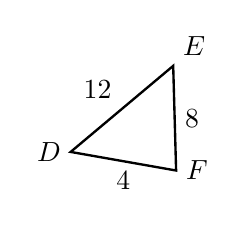
\begin{tikzpicture}

\def\len2{\lenA}

\draw[line width=0.3mm] (0,0) coordinate (d)  -- (40:\len2) coordinate (e) node[midway, anchor=south east, inner sep=0.07*\leninnersep, rotate=0] (12) {$ 12$} -- (-10:0.8*\len2) coordinate (f) node[midway, anchor=west, inner sep=0.07*\leninnersep, rotate=0] (8) {$ 8$} -- cycle node[midway, anchor=north, inner sep=0.07*\leninnersep, rotate=0] (4) {$ 4$}; 

\node[anchor=east, inner sep=0.07*\leninnersep, rotate=0] (d-label) at (d) {$ D$}; 

\node[anchor=south west, inner sep=0.07*\leninnersep, rotate=0] (e-label) at (e) {$ E$}; 

\node[anchor=west, inner sep=0.07*\leninnersep, rotate=0] (f-label) at (f) {$ F$}; 

\end{tikzpicture} 
%3
\item 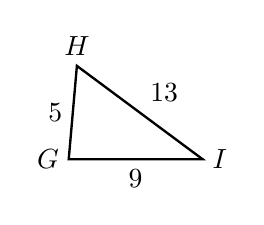
\begin{tikzpicture}

\def\len3{\lenA}

\draw[line width=0.3mm] (0,0) coordinate (g)  -- (85:0.7*\len3) coordinate (h) node[midway, anchor=east, inner sep=0.07*\leninnersep, rotate=0] (5) {$ 5$} -- (0:\len3) coordinate (i) node[midway, anchor=south west, inner sep=0.07*\leninnersep, rotate=0] (13) {$ 13$} -- cycle node[midway, anchor=north, inner sep=0.07*\leninnersep, rotate=0] (9) {$ 9$};  

\node[anchor=south, inner sep=0.07*\leninnersep, rotate=0] (h-label) at (h) {$ H$}; 

\node[anchor=east, inner sep=0.07*\leninnersep, rotate=0] (g-label) at (g) {$ G$}; 

\node[anchor=west, inner sep=0.07*\leninnersep, rotate=0] (i-label) at (i) {$ I$};

\end{tikzpicture} 
%4
\item 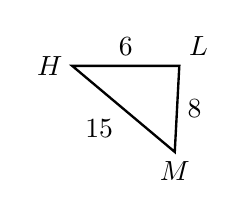
\begin{tikzpicture}

\def\len4{\lenA}

\draw[line width=0.3mm] (0,0) coordinate (h)  -- (0:0.8*\len4) coordinate (l) node[midway, anchor=south, inner sep=0.07*\leninnersep, rotate=0] (6) {$ 6$} -- (-40:\len4) coordinate (m) node[midway, anchor=west, inner sep=0.07*\leninnersep, rotate=0] (8) {$ 8$} -- cycle node[midway, anchor=north east, inner sep=0.07*\leninnersep, rotate=0] (15) {$ 15$}; 

\node[anchor=east, inner sep=0.07*\leninnersep, rotate=0] (h-label) at (h) {$ H$}; 

\node[anchor=south west, inner sep=0.07*\leninnersep, rotate=0] (l-label) at (l) {$ L$}; 

\node[anchor=north, inner sep=0.07*\leninnersep, rotate=0] (m-label) at (m) {$ M$}; 

\end{tikzpicture} 
\end{enumerate} 

\end{multicols} 
%B
\item \hspce Find the measure of the third angle of the triangle, then arrange the sides in increasing order. 

\begin{enumerate}[label = \arabic*. ]
%1
\item $m\angle{A} = 56\degree$; $ m\angle{B} = 87\degree$; $ m\angle{C} = \blank$
%2
\item $m\angle{P} = 106\degree$; $ m\angle{V} = 19\degree$; $ m\angle{C} = \blank$
%3
\item $m\angle{B} = 29\degree$; $ m\angle{P} = 72\degree$; $ m\angle{F} = \blank$
%4
\item $m\angle{G} = 97\degree$; $ m\angle{E} = 64\degree$; $ m\angle{O} = \blank$
%5
\item $m\angle{M} = 68\degree$; $ m\angle{A} = 22\degree$; $ m\angle{T} = \blank $
\end{enumerate} 
%C
\item \hspce Write \emph{Yes} if the given measure can form a triangle or \emph{No} if not. 

\vspace*{-0.75ex}

\begin{multicols}{2}

\begin{enumerate}[label = \arabic*. ]
%1
\item \hspce $8, 14, 9$
%2
\item \hspce $13, 25, 12$
%3
\item \hspce $3.6, 4.8, 9.0$
%4
\item \hspce $15, 20, 36$
%5
\item \hspce $6.5, 9.6, 2.9$ 

\end{enumerate}  

\end{multicols}



\end{enumerate} 


%\def\figdir{/storage/emulated/0/Documents/documents/latex/1920/Grade-8/3rd/inequalities-in-one-triangle/f}


\begin{enumerate}[label = \arabic*. ]
%D
\item[D. ] \hspce Give the range of the possible length of the third side of $\triangle ABC$. 

\vspace*{5ex}\hspace*{17em}\begin{tikzpicture}[remember picture, overlay] 

\def\len1{\lenA}

\draw[line width=0.3mm] (0,0) coordinate (b)  -- (50:0.6*\len1) coordinate (a) node[midway, anchor=south east, inner sep=0.07*\leninnersep, rotate=0] (c-mid) {$ c$} -- (0:\len1) coordinate (c) node[midway, anchor=south west, inner sep=0.07*\leninnersep, rotate=0] (b-mid) {$ b$} -- cycle node[midway, anchor=north, inner sep=0.07*\leninnersep, rotate=0] (a-mid) {$ a$}; 

\node[anchor=south, inner sep=0.07*\leninnersep, rotate=0] (a-label) at (a) {$ A$};

\node[anchor=east, inner sep=0.07*\leninnersep, rotate=0] (b-label) at (b) {$ B$};

\node[anchor=west, inner sep=0.07*\leninnersep, rotate=0] (c-label) at (c) {$ C$}; 

\end{tikzpicture} 
\vspace*{-7ex}

$
\begin{array}{llll}
1. \phantom{i} & a=9 & \phantom{mn} & b=7 \\
2. &	b=12 &	& c=29\\
3. &	a=15.2 &	& b=19.8 \\
4. & a=128.25 & & c=74.5 \\
5. &	a=3 \displaystyle \frac{2}{5} &	& c=2 \displaystyle \frac{1}{2}\\
\end{array}
$

%E
\item[E. ] \hspce Find the measure of the indicated angle. 
\begin{enumerate}[label = \arabic*. ]
%1
\item $m\angle{1} = 48\degree$; $m\angle{2} = 46\degree$; $ m\angle{4} = \blank$
%2
\item $m\angle{1} = 29\degree$; $ m\angle{2} = 52\degree$; $ m\angle{4} = \blank$
%3
\item $m\angle{2} = 18\degree$; $ m\angle{4} = 127\degree$; $ m\angle{1} = \blank$
%4
\item $m\angle{4} = 109\degree$; $ m\angle{1} = 86\degree$; $ m\angle{2} = \blank$
%5 
\item $m\angle{1} = (x+5)\degree$; $ m\angle{2} = (2x+51)\degree$; $ m\angle{4} = (5x-10)\degree$; $ x = \blank$
\end{enumerate}  
\end{enumerate}   

%\begin{center}

\vspace*{-19ex}\hspace*{22em}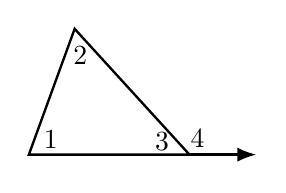
\begin{tikzpicture}

\def\len2{\lenA}

\draw[line width=0.3mm] (0,0) coordinate (1) node[yshift=-0.07*\leninnersep, inner sep=5pt, rotate=0, anchor=south west] (1-label) {$ 1$} -- (70:\len2) coordinate (2) node[xshift=2pt, inner sep=6pt, rotate=0, anchor=north] (2-label) {$ 2$} -- (0:1.2*\len2) coordinate (3) edge[-Latex] (0:1.7*\len2) node[yshift=-4pt, xshift=-2pt, inner sep=5pt, rotate=0, anchor=south east] (3-label) {$ 3$} node[yshift=0pt, xshift=-2pt, inner sep=2pt, rotate=0, anchor=south west] (4-label) {$ 4$}  -- cycle;  

\end{tikzpicture} 
\vspace*{4ex}

%\end{center} 
%\vspace*{1ex}
%\def\figdir{/storage/emulated/0/Documents/documents/latex/1920/Grade-8/3rd/inequalities-in-one-triangle/f}


%\textbf{Practice Exercises}
\textbf{Problem Set}

\vspce

\begin{enumerate}[label = \Alph*. ]
%A
\item \hspce Arrange the angles of the triangles in increasing order. 

\begin{multicols}{2}

\begin{enumerate}[label = \arabic*. ]
%1
\item 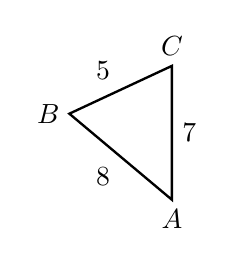
\begin{tikzpicture}

\def\len1{\lenA}

\draw[line width=0.3mm, rotate=90] (0,0) coordinate (a)  -- (50:\len1) coordinate (b) node[midway, anchor=north east, inner sep=0.07*\leninnersep, rotate=0] (8) {$ 8$} -- (0:\len1) coordinate (c) node[midway, anchor=south east, inner sep=0.07*\leninnersep, rotate=0] (5) {$ 5$}  -- cycle node[midway, anchor=west, inner sep=0.07*\leninnersep, rotate=0] (7) {$ 7$} ; 

\node[anchor=north, inner sep=0.07*\leninnersep, rotate=0] (a-label) at (a) {$ A$}; 

\node[anchor=east, inner sep=0.07*\leninnersep, rotate=0] (b-label) at (b) {$ B$}; 

\node[anchor=south, inner sep=0.07*\leninnersep, rotate=0] (c-label) at (c) {$ C$}; 

\end{tikzpicture} 
%2
\item 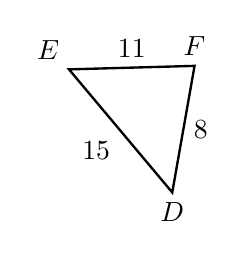
\begin{tikzpicture}

\def\len2{1.2*\lenA}

\draw[line width=0.3mm, rotate=90] (0,0) coordinate (d)  -- (40:\len2) coordinate (e) node[midway, anchor=north east, inner sep=0.07*\leninnersep, rotate=0] (15) {$ 15$} -- (-10:0.8*\len2) coordinate (f) node[midway, anchor=south, inner sep=0.07*\leninnersep, rotate=0] (11) {$ 11$} -- cycle node[midway, anchor=west, inner sep=0.07*\leninnersep, rotate=0] (4) {$ 8$}; 

\node[anchor=north, inner sep=0.07*\leninnersep, rotate=0] (d-label) at (d) {$ D$}; 

\node[anchor=south east, inner sep=0.07*\leninnersep, rotate=0] (e-label) at (e) {$ E$}; 

\node[anchor=south, inner sep=0.07*\leninnersep, rotate=0] (f-label) at (f) {$ F$}; 

\end{tikzpicture} 
%3
%\item 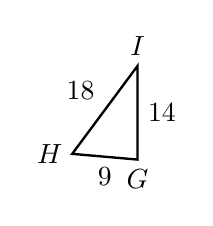
\begin{tikzpicture}

\def\len3{0.7*\lenA}

\draw[line width=0.3mm, rotate=90] (0,0) coordinate (g)  -- (85:0.7*\len3) coordinate (h) node[midway, anchor=north, inner sep=0.07*\leninnersep, rotate=0] (9) {$ 9$} -- (0:\len3) coordinate (i) node[midway, anchor=south east, inner sep=0.07*\leninnersep, rotate=0] (18) {$ 18$} -- cycle node[midway, anchor=west, inner sep=0.07*\leninnersep, rotate=0] (14) {$ 14$};  

\node[anchor=east, inner sep=0.07*\leninnersep, rotate=0] (h-label) at (h) {$ H$}; 

\node[anchor=north, inner sep=0.07*\leninnersep, rotate=0] (g-label) at (g) {$ G$}; 

\node[anchor=south, inner sep=0.07*\leninnersep, rotate=0] (i-label) at (i) {$ I$};

\end{tikzpicture} 
%4
%\item 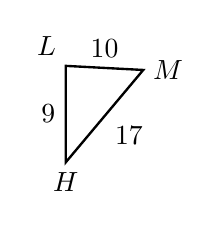
\begin{tikzpicture}

\def\len4{0.9*\lenA}

\draw[line width=0.3mm, rotate=90] (0,0) coordinate (h)  -- (0:0.8*\len4) coordinate (l) node[midway, anchor=east, inner sep=0.07*\leninnersep, rotate=0] (9) {$ 9$} -- (-40:\len4) coordinate (m) node[midway, anchor=south, inner sep=0.07*\leninnersep, rotate=0] (10) {$ 10$} -- cycle node[midway, anchor=north west, inner sep=0.07*\leninnersep, rotate=0] (17) {$ 17$}; 

\node[anchor=north, inner sep=0.07*\leninnersep, rotate=0] (h-label) at (h) {$ H$}; 

\node[anchor=south east, inner sep=0.07*\leninnersep, rotate=0] (l-label) at (l) {$ L$}; 

\node[anchor=west, inner sep=0.07*\leninnersep, rotate=0] (m-label) at (m) {$ M$}; 

\end{tikzpicture} 
\end{enumerate} 

\end{multicols} 
%B
\item \hspce Find the measure of the third angle of the triangle, then arrange the sides in increasing order. 

\begin{enumerate}[label = \arabic*. ]
%1
\item $m\angle{A} = 40\degree$; $ m\angle{B} = 89\degree$; $ m\angle{C} = \blank$
%2
\item $m\angle{P} = 117\degree$; $ m\angle{V} = 27\degree$; $ m\angle{C} = \blank$
%3
\item $m\angle{B} = 38\degree$; $ m\angle{P} = 92\degree$; $ m\angle{F} = \blank$
%4
%\item $m\angle{G} = 88\degree$; $ m\angle{E} = 71\degree$; $ m\angle{O} = \blank$
%5
%\item $m\angle{M} = 79\degree$; $ m\angle{A} = 35\degree$; $ m\angle{T} = \blank $
\end{enumerate} 
%C
\item \hspce Write \emph{Yes} if the given measure can form a triangle or \emph{No} if not. 

\vspace*{-0.75ex}

\begin{multicols}{3}

\begin{enumerate}[label = \arabic*. ]
%1
\item \hspce $6, 17, 12$
%2
\item \hspce $14, 33, 19$
%3
\item \hspce $3.7, 5.2, 8.5$
%4
%\item \hspce $27, 34, 49$
%5
%\item \hspce $6.5, 10.1, 3.6$ 

\end{enumerate}  

\end{multicols}

%D
\item \hspce Give the range of the possible length of the third side of $\triangle ABC$. 

\vspace*{4ex}\hspace*{15em}\begin{tikzpicture}[remember picture, overlay] 

\def\len1{\lenA}

\draw[line width=0.3mm] (0,0) coordinate (b)  -- (50:0.6*\len1) coordinate (a) node[midway, anchor=south east, inner sep=0.07*\leninnersep, rotate=0] (c-mid) {$ c$} -- (0:\len1) coordinate (c) node[midway, anchor=south west, inner sep=0.07*\leninnersep, rotate=0] (b-mid) {$ b$} -- cycle node[midway, anchor=north, inner sep=0.07*\leninnersep, rotate=0] (a-mid) {$ a$}; 

\node[anchor=south, inner sep=0.07*\leninnersep, rotate=0] (a-label) at (a) {$ A$};

\node[anchor=east, inner sep=0.07*\leninnersep, rotate=0] (b-label) at (b) {$ B$};

\node[anchor=west, inner sep=0.07*\leninnersep, rotate=0] (c-label) at (c) {$ C$}; 

\end{tikzpicture} 
\vspace*{-6ex}


$
\begin{array}{llll}
1. \phantom{i} & a=5 & \phantom{mn} & b=12 \\
%2. &	b=18 &	& c=23\\
2. &	a=17.4 &	& b=28.1 \\
%4. & a=107.4 & & c=74.35 \\
3. &	a=7 \displaystyle \frac{1}{4} &	& c=3 \displaystyle \frac{1}{2}\\
\end{array}
$

%E
\item \hspce Find the measure of the indicated angle. 
\begin{enumerate}[label = \arabic*. ]
%1
\item $m\angle{1} = 57\degree$; $m\angle{2} = 54\degree$; $ m\angle{4} = \blank$
%2
%\item $m\angle{1} = 43\degree$; $ m\angle{2} = 65\degree$; $ m\angle{4} = \blank$
%3
\item $m\angle{2} = 37\degree$; $ m\angle{4} = 150\degree$; $ m\angle{1} = \blank$
%4
%\item $m\angle{4} = 132\degree$; $ m\angle{1} = 76\degree$; $ m\angle{2} = \blank$
%5 
\item $m\angle{1} = (2x+7)\degree$; $ m\angle{2} = (x+31)\degree$; $ m\angle{4} = (6x-4)\degree$; $ x = \blank$
\end{enumerate}  

\end{enumerate} 

\vspace*{-16ex}\hspace*{22em}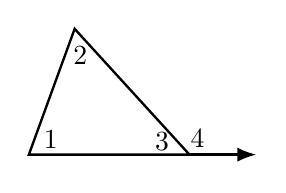
\begin{tikzpicture}

\def\len2{\lenA}

\draw[line width=0.3mm] (0,0) coordinate (1) node[yshift=-0.07*\leninnersep, inner sep=5pt, rotate=0, anchor=south west] (1-label) {$ 1$} -- (70:\len2) coordinate (2) node[xshift=2pt, inner sep=6pt, rotate=0, anchor=north] (2-label) {$ 2$} -- (0:1.2*\len2) coordinate (3) edge[-Latex] (0:1.7*\len2) node[yshift=-4pt, xshift=-2pt, inner sep=5pt, rotate=0, anchor=south east] (3-label) {$ 3$} node[yshift=0pt, xshift=-2pt, inner sep=2pt, rotate=0, anchor=south west] (4-label) {$ 4$}  -- cycle;  

\end{tikzpicture} 
\vspace*{4ex}

\end{frame}

% frame 4
\vertadjustb
\begin{frame} 
%\begin{center}
\textbf{Inequalities in One Triangle 
}
\end{center}

\vspce
Unequal Sides Theorem: 
 If the lengths of the sides of a triangle are not equal, then the angles opposite these sides are also not equal and the larger angle is opposite the longer side.
 
\vspce 

Unequal Angles Theorem: If the measure of the three angles of a triangle is not equal, the sides opposite the angles are also not equal and the longer side is opposite the larger angle. 

\vspce 

Triangle Inequality Theorem: The sum of the length of the two sides of a triangle is greater than the third side.

\vspce 

The Exterior Angle Theorem 1: The measure of an exterior angle of a triangle is greater than the measure of either remote interior angle.

\vspce 

The Exterior Angle Theorem 2: The measure of the exterior angle of a triangle is equal to the sum of the measures of the two remote interior angles. 
%\def\figdir{/storage/emulated/0/Documents/documents/latex/1920/Grade-8/3rd/inequalities-in-one-triangle/f}

\textbf{Practice Exercises}
%\textbf{Problem Set}

\vspce

\begin{enumerate}[label = \Alph*. ]
%A
\item \hspce Arrange the angles of the triangles in increasing order. 

\begin{multicols}{2}

\begin{enumerate}[label = \arabic*. ]
%1
\item 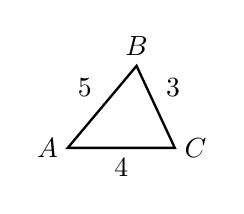
\begin{tikzpicture}

\def\len1{0.8*\lenA}

\draw[line width=0.3mm] (0,0) coordinate (a)  -- (50:\len1) coordinate (b) node[midway, anchor=south east, inner sep=0.07*\leninnersep, rotate=0] (5) {$ 5$} -- (0:\len1) coordinate (c) node[midway, anchor=south west, inner sep=0.07*\leninnersep, rotate=0] (3) {$ 3$}  -- cycle node[midway, anchor=north, inner sep=0.07*\leninnersep, rotate=0] (4) {$ 4$} ; 

\node[anchor=east, inner sep=0.07*\leninnersep, rotate=0] (a-label) at (a) {$ A$}; 

\node[anchor=south, inner sep=0.07*\leninnersep, rotate=0] (b-label) at (b) {$ B$}; 

\node[anchor=west, inner sep=0.07*\leninnersep, rotate=0] (c-label) at (c) {$ C$}; 

\end{tikzpicture} 
%2
\item 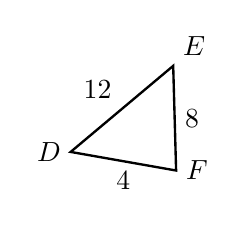
\begin{tikzpicture}

\def\len2{\lenA}

\draw[line width=0.3mm] (0,0) coordinate (d)  -- (40:\len2) coordinate (e) node[midway, anchor=south east, inner sep=0.07*\leninnersep, rotate=0] (12) {$ 12$} -- (-10:0.8*\len2) coordinate (f) node[midway, anchor=west, inner sep=0.07*\leninnersep, rotate=0] (8) {$ 8$} -- cycle node[midway, anchor=north, inner sep=0.07*\leninnersep, rotate=0] (4) {$ 4$}; 

\node[anchor=east, inner sep=0.07*\leninnersep, rotate=0] (d-label) at (d) {$ D$}; 

\node[anchor=south west, inner sep=0.07*\leninnersep, rotate=0] (e-label) at (e) {$ E$}; 

\node[anchor=west, inner sep=0.07*\leninnersep, rotate=0] (f-label) at (f) {$ F$}; 

\end{tikzpicture} 
%3
\item 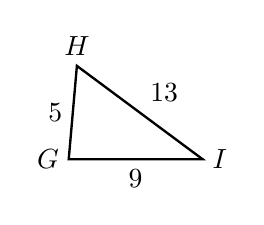
\begin{tikzpicture}

\def\len3{\lenA}

\draw[line width=0.3mm] (0,0) coordinate (g)  -- (85:0.7*\len3) coordinate (h) node[midway, anchor=east, inner sep=0.07*\leninnersep, rotate=0] (5) {$ 5$} -- (0:\len3) coordinate (i) node[midway, anchor=south west, inner sep=0.07*\leninnersep, rotate=0] (13) {$ 13$} -- cycle node[midway, anchor=north, inner sep=0.07*\leninnersep, rotate=0] (9) {$ 9$};  

\node[anchor=south, inner sep=0.07*\leninnersep, rotate=0] (h-label) at (h) {$ H$}; 

\node[anchor=east, inner sep=0.07*\leninnersep, rotate=0] (g-label) at (g) {$ G$}; 

\node[anchor=west, inner sep=0.07*\leninnersep, rotate=0] (i-label) at (i) {$ I$};

\end{tikzpicture} 
%4
\item 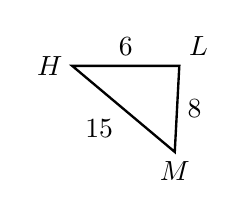
\begin{tikzpicture}

\def\len4{\lenA}

\draw[line width=0.3mm] (0,0) coordinate (h)  -- (0:0.8*\len4) coordinate (l) node[midway, anchor=south, inner sep=0.07*\leninnersep, rotate=0] (6) {$ 6$} -- (-40:\len4) coordinate (m) node[midway, anchor=west, inner sep=0.07*\leninnersep, rotate=0] (8) {$ 8$} -- cycle node[midway, anchor=north east, inner sep=0.07*\leninnersep, rotate=0] (15) {$ 15$}; 

\node[anchor=east, inner sep=0.07*\leninnersep, rotate=0] (h-label) at (h) {$ H$}; 

\node[anchor=south west, inner sep=0.07*\leninnersep, rotate=0] (l-label) at (l) {$ L$}; 

\node[anchor=north, inner sep=0.07*\leninnersep, rotate=0] (m-label) at (m) {$ M$}; 

\end{tikzpicture} 
\end{enumerate} 

\end{multicols} 
%B
\item \hspce Find the measure of the third angle of the triangle, then arrange the sides in increasing order. 

\begin{enumerate}[label = \arabic*. ]
%1
\item $m\angle{A} = 56\degree$; $ m\angle{B} = 87\degree$; $ m\angle{C} = \blank$
%2
\item $m\angle{P} = 106\degree$; $ m\angle{V} = 19\degree$; $ m\angle{C} = \blank$
%3
\item $m\angle{B} = 29\degree$; $ m\angle{P} = 72\degree$; $ m\angle{F} = \blank$
%4
\item $m\angle{G} = 97\degree$; $ m\angle{E} = 64\degree$; $ m\angle{O} = \blank$
%5
\item $m\angle{M} = 68\degree$; $ m\angle{A} = 22\degree$; $ m\angle{T} = \blank $
\end{enumerate} 
%C
\item \hspce Write \emph{Yes} if the given measure can form a triangle or \emph{No} if not. 

\vspace*{-0.75ex}

\begin{multicols}{2}

\begin{enumerate}[label = \arabic*. ]
%1
\item \hspce $8, 14, 9$
%2
\item \hspce $13, 25, 12$
%3
\item \hspce $3.6, 4.8, 9.0$
%4
\item \hspce $15, 20, 36$
%5
\item \hspce $6.5, 9.6, 2.9$ 

\end{enumerate}  

\end{multicols}



\end{enumerate} 


\def\figdir{/storage/emulated/0/Documents/documents/latex/1920/Grade-8/3rd/inequalities-in-one-triangle/f}


\begin{enumerate}[label = \arabic*. ]
%D
\item[D. ] \hspce Give the range of the possible length of the third side of $\triangle ABC$. 

\vspace*{5ex}\hspace*{17em}\begin{tikzpicture}[remember picture, overlay] 

\def\len1{\lenA}

\draw[line width=0.3mm] (0,0) coordinate (b)  -- (50:0.6*\len1) coordinate (a) node[midway, anchor=south east, inner sep=0.07*\leninnersep, rotate=0] (c-mid) {$ c$} -- (0:\len1) coordinate (c) node[midway, anchor=south west, inner sep=0.07*\leninnersep, rotate=0] (b-mid) {$ b$} -- cycle node[midway, anchor=north, inner sep=0.07*\leninnersep, rotate=0] (a-mid) {$ a$}; 

\node[anchor=south, inner sep=0.07*\leninnersep, rotate=0] (a-label) at (a) {$ A$};

\node[anchor=east, inner sep=0.07*\leninnersep, rotate=0] (b-label) at (b) {$ B$};

\node[anchor=west, inner sep=0.07*\leninnersep, rotate=0] (c-label) at (c) {$ C$}; 

\end{tikzpicture} 
\vspace*{-7ex}

$
\begin{array}{llll}
1. \phantom{i} & a=9 & \phantom{mn} & b=7 \\
2. &	b=12 &	& c=29\\
3. &	a=15.2 &	& b=19.8 \\
4. & a=128.25 & & c=74.5 \\
5. &	a=3 \displaystyle \frac{2}{5} &	& c=2 \displaystyle \frac{1}{2}\\
\end{array}
$

%E
\item[E. ] \hspce Find the measure of the indicated angle. 
\begin{enumerate}[label = \arabic*. ]
%1
\item $m\angle{1} = 48\degree$; $m\angle{2} = 46\degree$; $ m\angle{4} = \blank$
%2
\item $m\angle{1} = 29\degree$; $ m\angle{2} = 52\degree$; $ m\angle{4} = \blank$
%3
\item $m\angle{2} = 18\degree$; $ m\angle{4} = 127\degree$; $ m\angle{1} = \blank$
%4
\item $m\angle{4} = 109\degree$; $ m\angle{1} = 86\degree$; $ m\angle{2} = \blank$
%5 
\item $m\angle{1} = (x+5)\degree$; $ m\angle{2} = (2x+51)\degree$; $ m\angle{4} = (5x-10)\degree$; $ x = \blank$
\end{enumerate}  
\end{enumerate}   

%\begin{center}

\vspace*{-19ex}\hspace*{22em}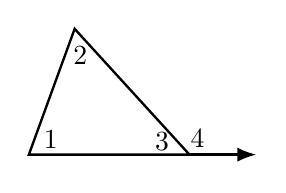
\begin{tikzpicture}

\def\len2{\lenA}

\draw[line width=0.3mm] (0,0) coordinate (1) node[yshift=-0.07*\leninnersep, inner sep=5pt, rotate=0, anchor=south west] (1-label) {$ 1$} -- (70:\len2) coordinate (2) node[xshift=2pt, inner sep=6pt, rotate=0, anchor=north] (2-label) {$ 2$} -- (0:1.2*\len2) coordinate (3) edge[-Latex] (0:1.7*\len2) node[yshift=-4pt, xshift=-2pt, inner sep=5pt, rotate=0, anchor=south east] (3-label) {$ 3$} node[yshift=0pt, xshift=-2pt, inner sep=2pt, rotate=0, anchor=south west] (4-label) {$ 4$}  -- cycle;  

\end{tikzpicture} 
\vspace*{4ex}

%\end{center} 
%\input{hand-inequalities-in-one-triangle-input2}
\vspace*{1ex}
\def\figdir{/storage/emulated/0/Documents/documents/latex/1920/Grade-8/3rd/inequalities-in-one-triangle/f}


%\textbf{Practice Exercises}
\textbf{Problem Set}

\vspce

\begin{enumerate}[label = \Alph*. ]
%A
\item \hspce Arrange the angles of the triangles in increasing order. 

\begin{multicols}{2}

\begin{enumerate}[label = \arabic*. ]
%1
\item 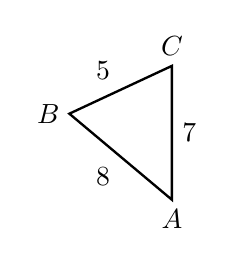
\begin{tikzpicture}

\def\len1{\lenA}

\draw[line width=0.3mm, rotate=90] (0,0) coordinate (a)  -- (50:\len1) coordinate (b) node[midway, anchor=north east, inner sep=0.07*\leninnersep, rotate=0] (8) {$ 8$} -- (0:\len1) coordinate (c) node[midway, anchor=south east, inner sep=0.07*\leninnersep, rotate=0] (5) {$ 5$}  -- cycle node[midway, anchor=west, inner sep=0.07*\leninnersep, rotate=0] (7) {$ 7$} ; 

\node[anchor=north, inner sep=0.07*\leninnersep, rotate=0] (a-label) at (a) {$ A$}; 

\node[anchor=east, inner sep=0.07*\leninnersep, rotate=0] (b-label) at (b) {$ B$}; 

\node[anchor=south, inner sep=0.07*\leninnersep, rotate=0] (c-label) at (c) {$ C$}; 

\end{tikzpicture} 
%2
\item 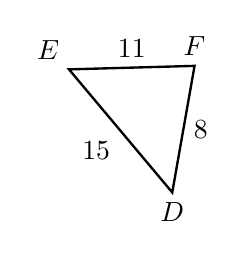
\begin{tikzpicture}

\def\len2{1.2*\lenA}

\draw[line width=0.3mm, rotate=90] (0,0) coordinate (d)  -- (40:\len2) coordinate (e) node[midway, anchor=north east, inner sep=0.07*\leninnersep, rotate=0] (15) {$ 15$} -- (-10:0.8*\len2) coordinate (f) node[midway, anchor=south, inner sep=0.07*\leninnersep, rotate=0] (11) {$ 11$} -- cycle node[midway, anchor=west, inner sep=0.07*\leninnersep, rotate=0] (4) {$ 8$}; 

\node[anchor=north, inner sep=0.07*\leninnersep, rotate=0] (d-label) at (d) {$ D$}; 

\node[anchor=south east, inner sep=0.07*\leninnersep, rotate=0] (e-label) at (e) {$ E$}; 

\node[anchor=south, inner sep=0.07*\leninnersep, rotate=0] (f-label) at (f) {$ F$}; 

\end{tikzpicture} 
%3
%\item 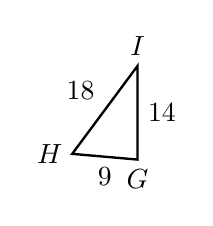
\begin{tikzpicture}

\def\len3{0.7*\lenA}

\draw[line width=0.3mm, rotate=90] (0,0) coordinate (g)  -- (85:0.7*\len3) coordinate (h) node[midway, anchor=north, inner sep=0.07*\leninnersep, rotate=0] (9) {$ 9$} -- (0:\len3) coordinate (i) node[midway, anchor=south east, inner sep=0.07*\leninnersep, rotate=0] (18) {$ 18$} -- cycle node[midway, anchor=west, inner sep=0.07*\leninnersep, rotate=0] (14) {$ 14$};  

\node[anchor=east, inner sep=0.07*\leninnersep, rotate=0] (h-label) at (h) {$ H$}; 

\node[anchor=north, inner sep=0.07*\leninnersep, rotate=0] (g-label) at (g) {$ G$}; 

\node[anchor=south, inner sep=0.07*\leninnersep, rotate=0] (i-label) at (i) {$ I$};

\end{tikzpicture} 
%4
%\item 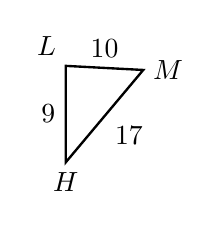
\begin{tikzpicture}

\def\len4{0.9*\lenA}

\draw[line width=0.3mm, rotate=90] (0,0) coordinate (h)  -- (0:0.8*\len4) coordinate (l) node[midway, anchor=east, inner sep=0.07*\leninnersep, rotate=0] (9) {$ 9$} -- (-40:\len4) coordinate (m) node[midway, anchor=south, inner sep=0.07*\leninnersep, rotate=0] (10) {$ 10$} -- cycle node[midway, anchor=north west, inner sep=0.07*\leninnersep, rotate=0] (17) {$ 17$}; 

\node[anchor=north, inner sep=0.07*\leninnersep, rotate=0] (h-label) at (h) {$ H$}; 

\node[anchor=south east, inner sep=0.07*\leninnersep, rotate=0] (l-label) at (l) {$ L$}; 

\node[anchor=west, inner sep=0.07*\leninnersep, rotate=0] (m-label) at (m) {$ M$}; 

\end{tikzpicture} 
\end{enumerate} 

\end{multicols} 
%B
\item \hspce Find the measure of the third angle of the triangle, then arrange the sides in increasing order. 

\begin{enumerate}[label = \arabic*. ]
%1
\item $m\angle{A} = 40\degree$; $ m\angle{B} = 89\degree$; $ m\angle{C} = \blank$
%2
\item $m\angle{P} = 117\degree$; $ m\angle{V} = 27\degree$; $ m\angle{C} = \blank$
%3
\item $m\angle{B} = 38\degree$; $ m\angle{P} = 92\degree$; $ m\angle{F} = \blank$
%4
%\item $m\angle{G} = 88\degree$; $ m\angle{E} = 71\degree$; $ m\angle{O} = \blank$
%5
%\item $m\angle{M} = 79\degree$; $ m\angle{A} = 35\degree$; $ m\angle{T} = \blank $
\end{enumerate} 
%C
\item \hspce Write \emph{Yes} if the given measure can form a triangle or \emph{No} if not. 

\vspace*{-0.75ex}

\begin{multicols}{3}

\begin{enumerate}[label = \arabic*. ]
%1
\item \hspce $6, 17, 12$
%2
\item \hspce $14, 33, 19$
%3
\item \hspce $3.7, 5.2, 8.5$
%4
%\item \hspce $27, 34, 49$
%5
%\item \hspce $6.5, 10.1, 3.6$ 

\end{enumerate}  

\end{multicols}

%D
\item \hspce Give the range of the possible length of the third side of $\triangle ABC$. 

\vspace*{4ex}\hspace*{15em}\begin{tikzpicture}[remember picture, overlay] 

\def\len1{\lenA}

\draw[line width=0.3mm] (0,0) coordinate (b)  -- (50:0.6*\len1) coordinate (a) node[midway, anchor=south east, inner sep=0.07*\leninnersep, rotate=0] (c-mid) {$ c$} -- (0:\len1) coordinate (c) node[midway, anchor=south west, inner sep=0.07*\leninnersep, rotate=0] (b-mid) {$ b$} -- cycle node[midway, anchor=north, inner sep=0.07*\leninnersep, rotate=0] (a-mid) {$ a$}; 

\node[anchor=south, inner sep=0.07*\leninnersep, rotate=0] (a-label) at (a) {$ A$};

\node[anchor=east, inner sep=0.07*\leninnersep, rotate=0] (b-label) at (b) {$ B$};

\node[anchor=west, inner sep=0.07*\leninnersep, rotate=0] (c-label) at (c) {$ C$}; 

\end{tikzpicture} 
\vspace*{-6ex}


$
\begin{array}{llll}
1. \phantom{i} & a=5 & \phantom{mn} & b=12 \\
%2. &	b=18 &	& c=23\\
2. &	a=17.4 &	& b=28.1 \\
%4. & a=107.4 & & c=74.35 \\
3. &	a=7 \displaystyle \frac{1}{4} &	& c=3 \displaystyle \frac{1}{2}\\
\end{array}
$

%E
\item \hspce Find the measure of the indicated angle. 
\begin{enumerate}[label = \arabic*. ]
%1
\item $m\angle{1} = 57\degree$; $m\angle{2} = 54\degree$; $ m\angle{4} = \blank$
%2
%\item $m\angle{1} = 43\degree$; $ m\angle{2} = 65\degree$; $ m\angle{4} = \blank$
%3
\item $m\angle{2} = 37\degree$; $ m\angle{4} = 150\degree$; $ m\angle{1} = \blank$
%4
%\item $m\angle{4} = 132\degree$; $ m\angle{1} = 76\degree$; $ m\angle{2} = \blank$
%5 
\item $m\angle{1} = (2x+7)\degree$; $ m\angle{2} = (x+31)\degree$; $ m\angle{4} = (6x-4)\degree$; $ x = \blank$
\end{enumerate}  

\end{enumerate} 

\vspace*{-16ex}\hspace*{22em}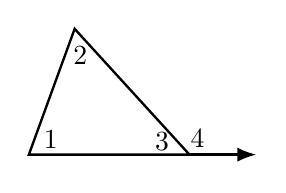
\begin{tikzpicture}

\def\len2{\lenA}

\draw[line width=0.3mm] (0,0) coordinate (1) node[yshift=-0.07*\leninnersep, inner sep=5pt, rotate=0, anchor=south west] (1-label) {$ 1$} -- (70:\len2) coordinate (2) node[xshift=2pt, inner sep=6pt, rotate=0, anchor=north] (2-label) {$ 2$} -- (0:1.2*\len2) coordinate (3) edge[-Latex] (0:1.7*\len2) node[yshift=-4pt, xshift=-2pt, inner sep=5pt, rotate=0, anchor=south east] (3-label) {$ 3$} node[yshift=0pt, xshift=-2pt, inner sep=2pt, rotate=0, anchor=south west] (4-label) {$ 4$}  -- cycle;  

\end{tikzpicture} 
\vspace*{4ex}


\end{frame}

\end{document}

